\chapter{Missions}

\startcontents[chapters]
\printmyminitoc{
This chapter will specify my roles and responsibilities in the position as a data scientist apprentice at SFR. Additionally, it will introduce the problems that I need to solve and the objective of each mission that I need to achieve at the end of the apprenticeship duration. The details of techniques, the methods that I used, and also the results will be discussed in the next chapter, \autoref{chap:problemsolving}. The current chapter centers on the introduction of the problems and the desired outcomes only.
}

The data science team at SFR Analytics contributes to a wide array of crucial tasks aimed at using the power of data for informed decision-making and strategic insights. The diverse responsibilities of our team contain, but are not limited to, the following:

\begin{itemize}
    \item Data Collection

    Gather, process, and clean large datasets from various sources, including customer interactions, network performance metrics, and user behavior data.
    
    \item Data Exploration

    Conduct data exploration to identify trends, patterns, and insights that can inform business strategies and improve operations.
    
    \item Predictive Modeling and Machine Learning

    Develop and implement machine learning models to predict customer behavior, optimize network performance, reduce churn rate and drive various business outcomes.
    
    \item Impact Assessment and Strategy

    Measure the impact of data science initiatives on key performance indicators and contribute to the development of business strategies.
\end{itemize}

As part of the Data Science team, each member is assigned specific responsibilities aligned with their expertise and the organization's goals. Together with other teams, we contribute to the company using data-driven techniques to improve efficiency and productivity.

\section{Roles and position}

As a data scientist at the Data Science Team of SFR Analytics, I contribute to the company's data-driven decision-making processes and strategic initiatives. SFR is committed to delivering cutting-edge communication and connectivity services to its diverse customers. In line with this mission, SFR Analytics serves as the analytical arm of the organization, dedicated to extracting valuable insights from the vast volumes of data generated within the telecommunications landscape.

Within this context, my assignment centers on these 3 main problems:

\begin{itemize}
    \item Improve fake and near-duplicate fiber distribution point image detection.
    \item Research the feasibility of moving existing infrastructure to Google Cloud.
    \item Categorize topics from the conversation with customers from the call center using NLP techniques.
\end{itemize}

These problems have been identified as necessary and, once addressed, have the potential to drive a positive impact for both SFR and its customers.

Throughout my period as an apprentice in the company, my duty in the team changed through time, from improving existing models to doing research and reporting on the feasibility of bringing existing infrastructure to the cloud, as well as creating new directions for the group in the future.


\section{In charge projects}

\subsection{Fiber distribution point fake and near-duplicated images detection}

SFR and other operators (Orange, Free and Bouygues) have a network of fiber aggregation points all over France. Because of the size of the network, the expense of maintenance and modernization is huge. In order to reduce the cost, It is more optimized to collaborate and share the network between operators. Orange, Free and Bouygues can use SFR fiber distribution points and vice versa.

\begin{figure}[H]
    \centering
    \begin{subfigure}{0.3\textwidth}
        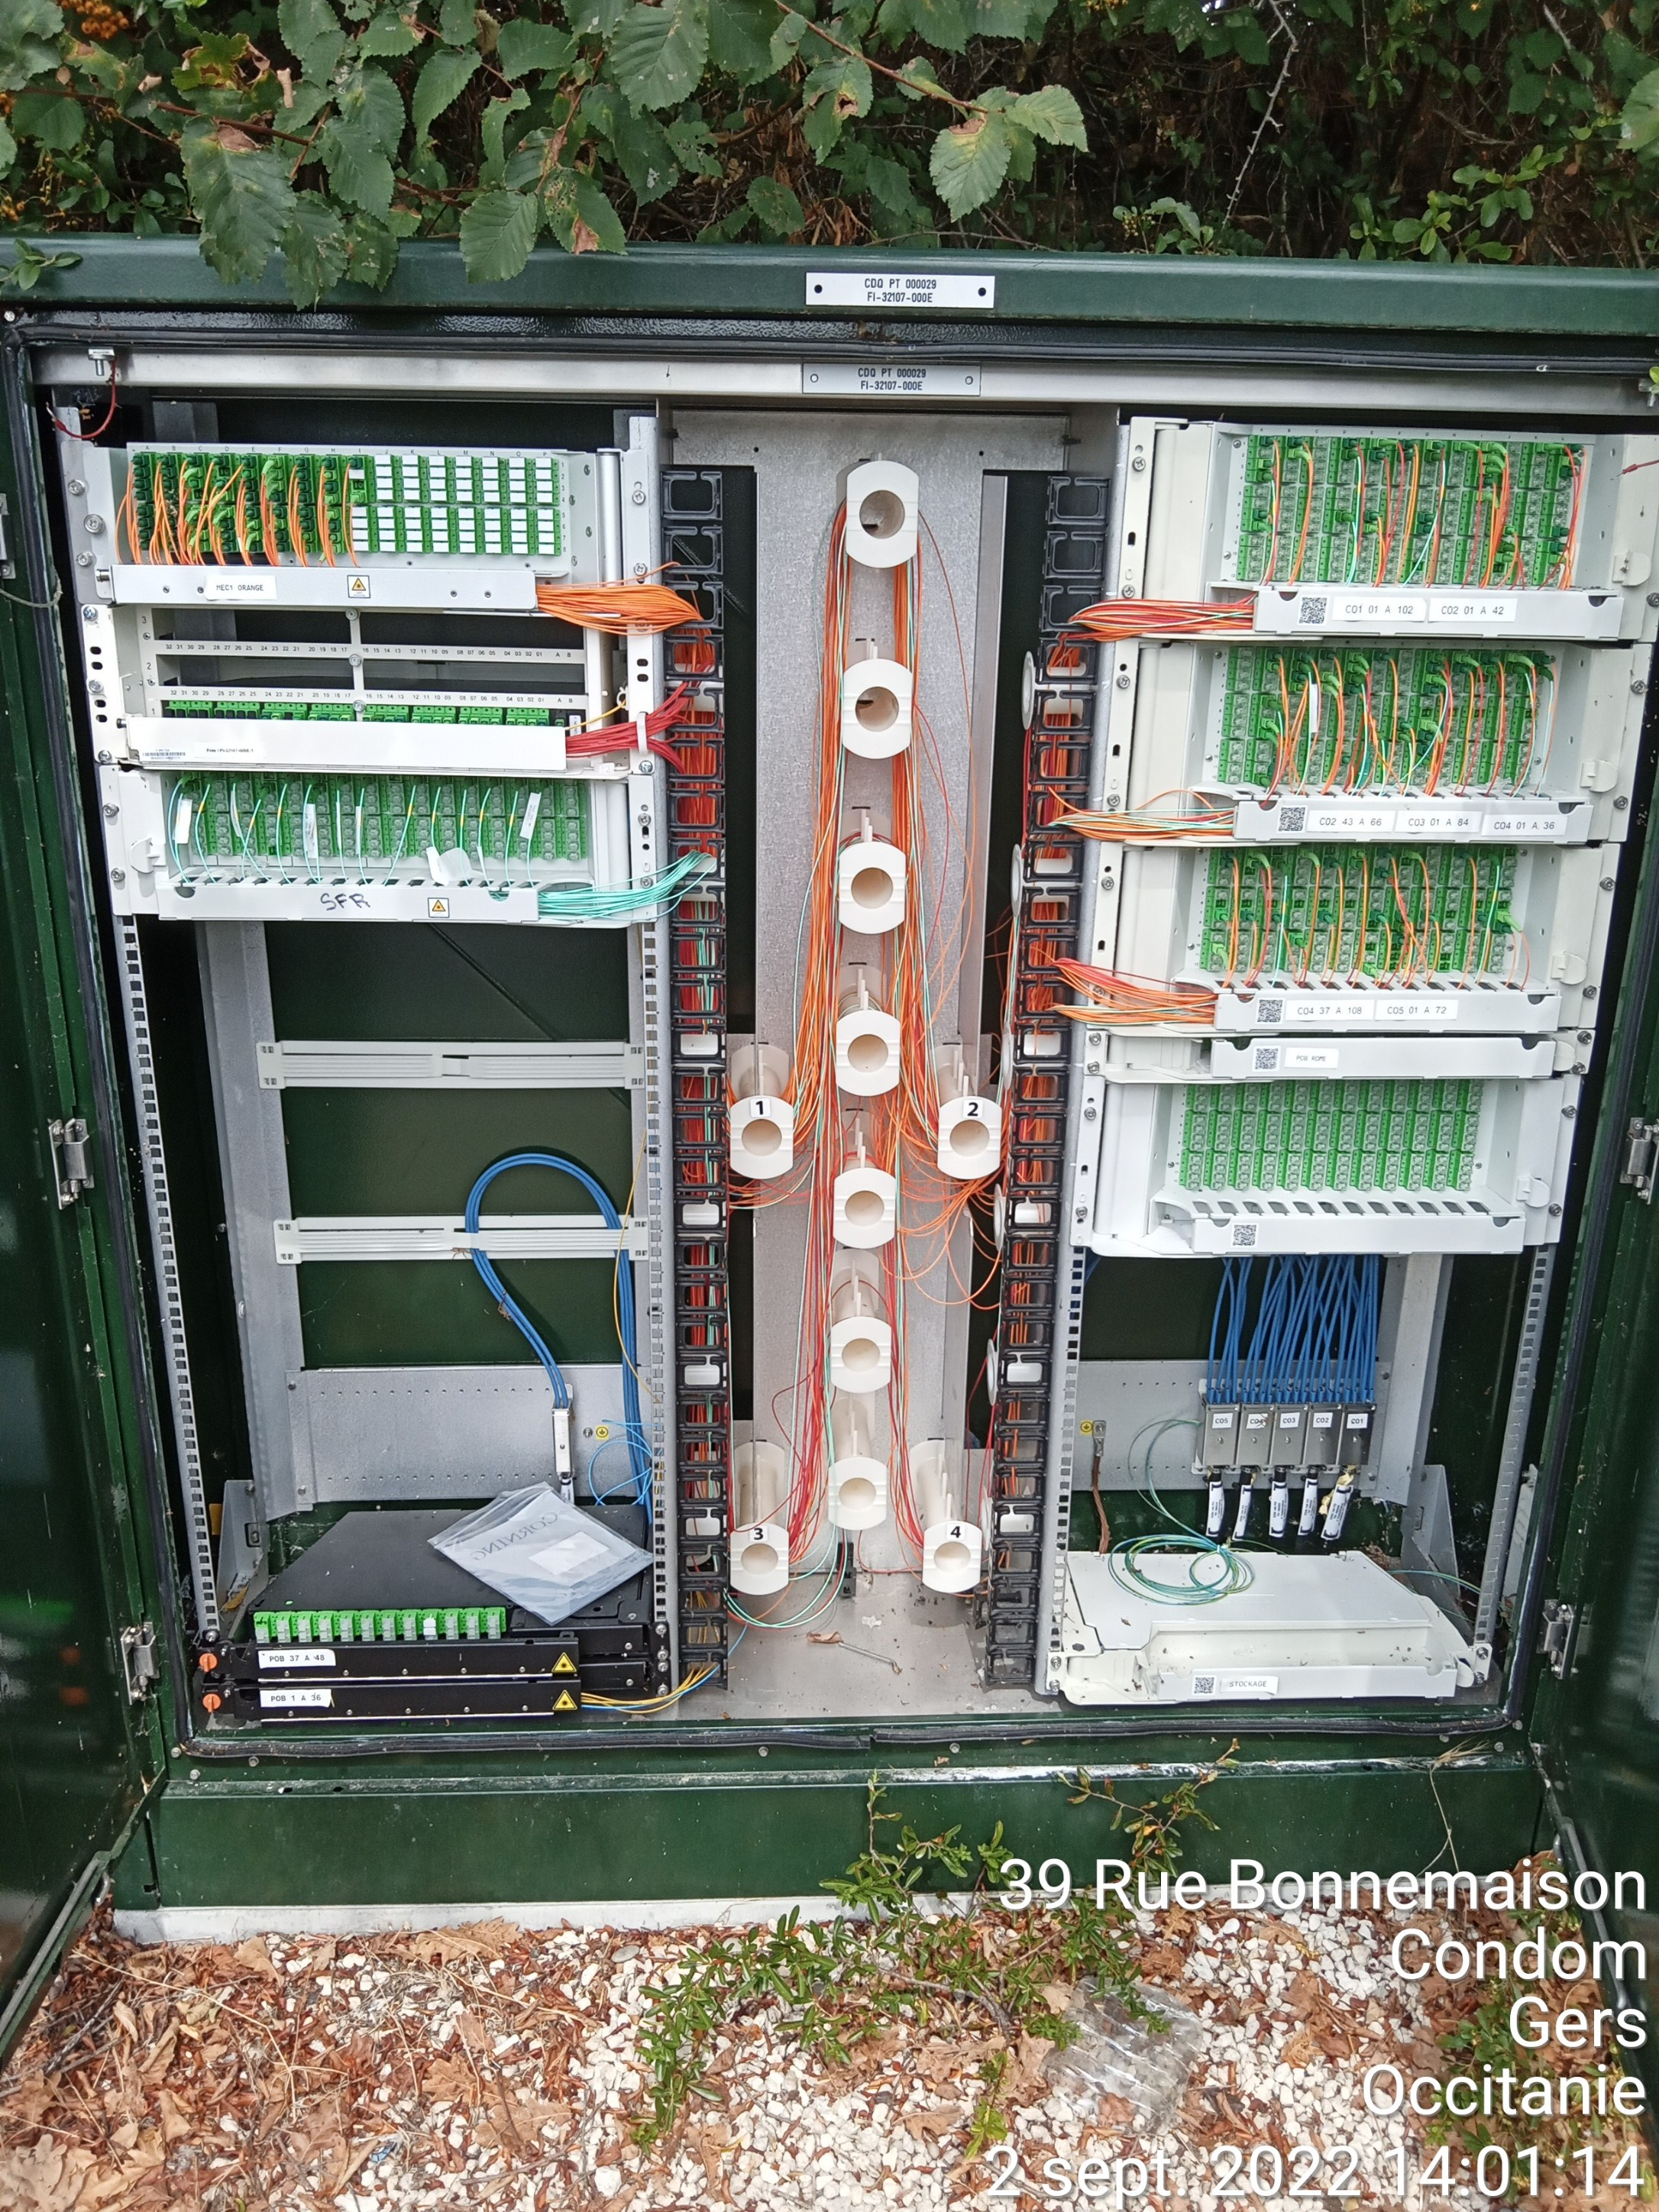
\includegraphics[width=\linewidth]{images/pm_example.jpg}
        \caption{PM no 1}
    \end{subfigure}
    \begin{subfigure}{0.3\textwidth}
        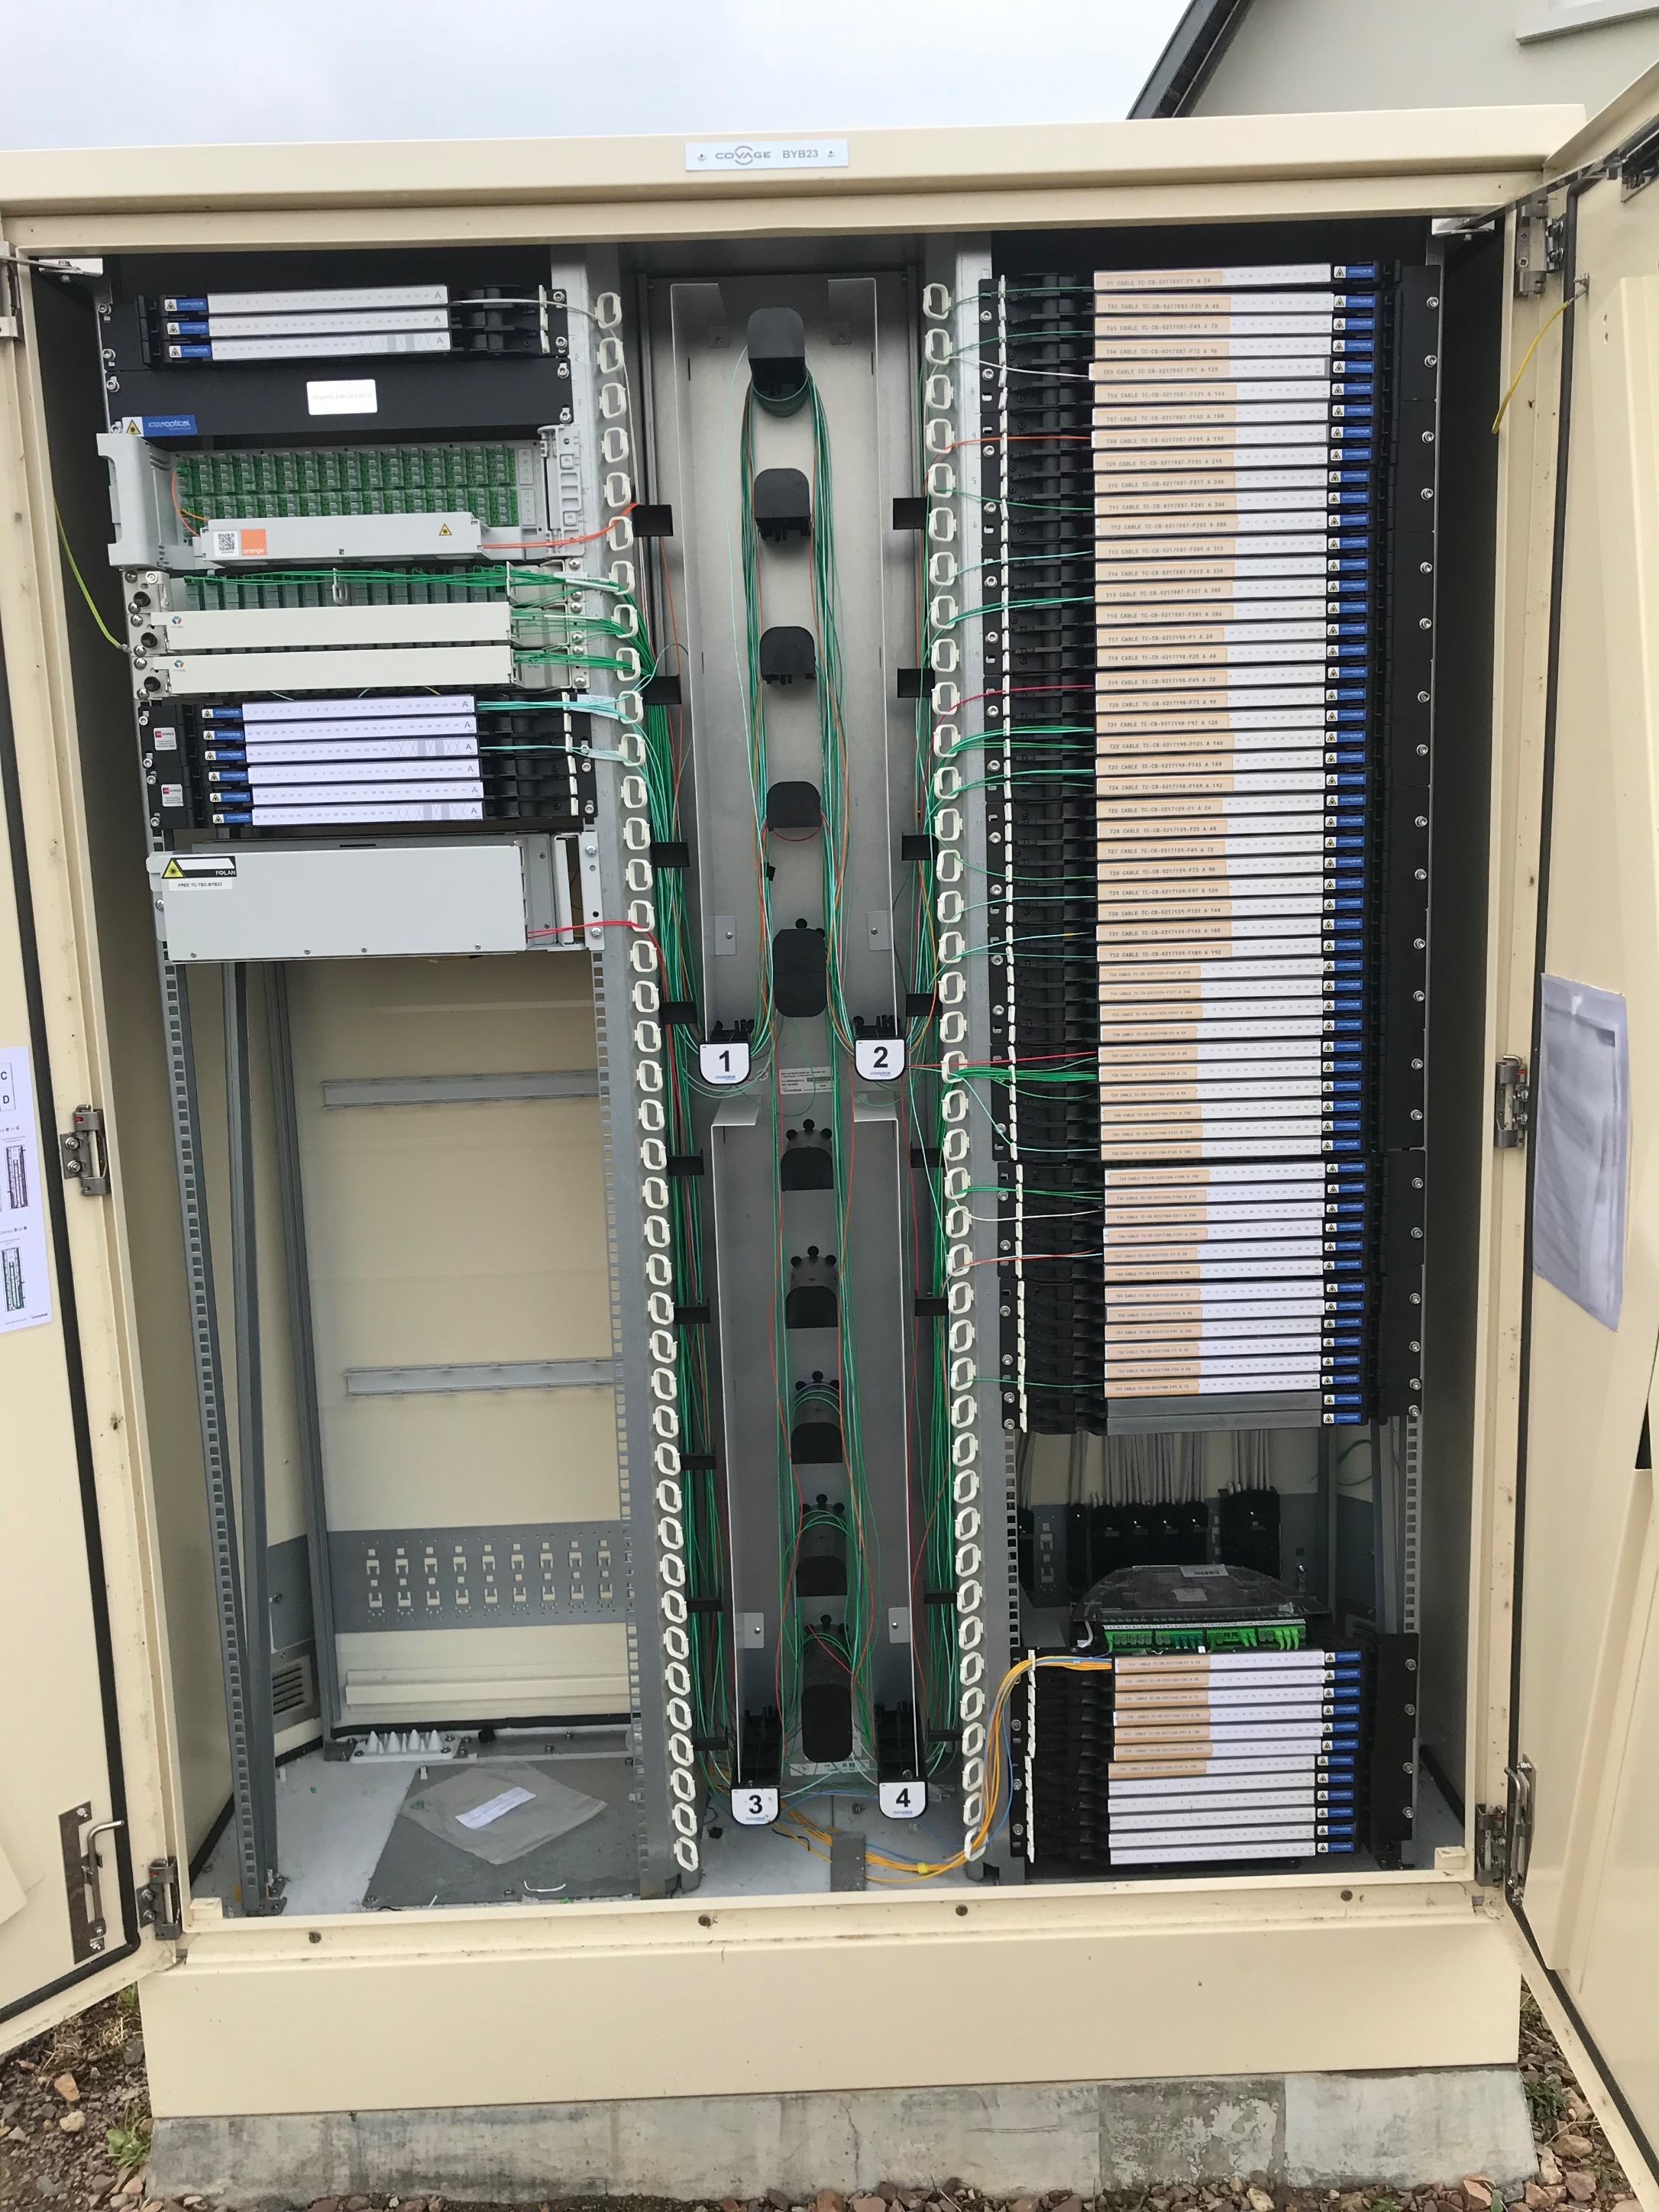
\includegraphics[width=\linewidth]{images/pm_example_2.jpg}
        \caption{PM no 2}
    \end{subfigure}
    \begin{subfigure}{0.3\textwidth}
        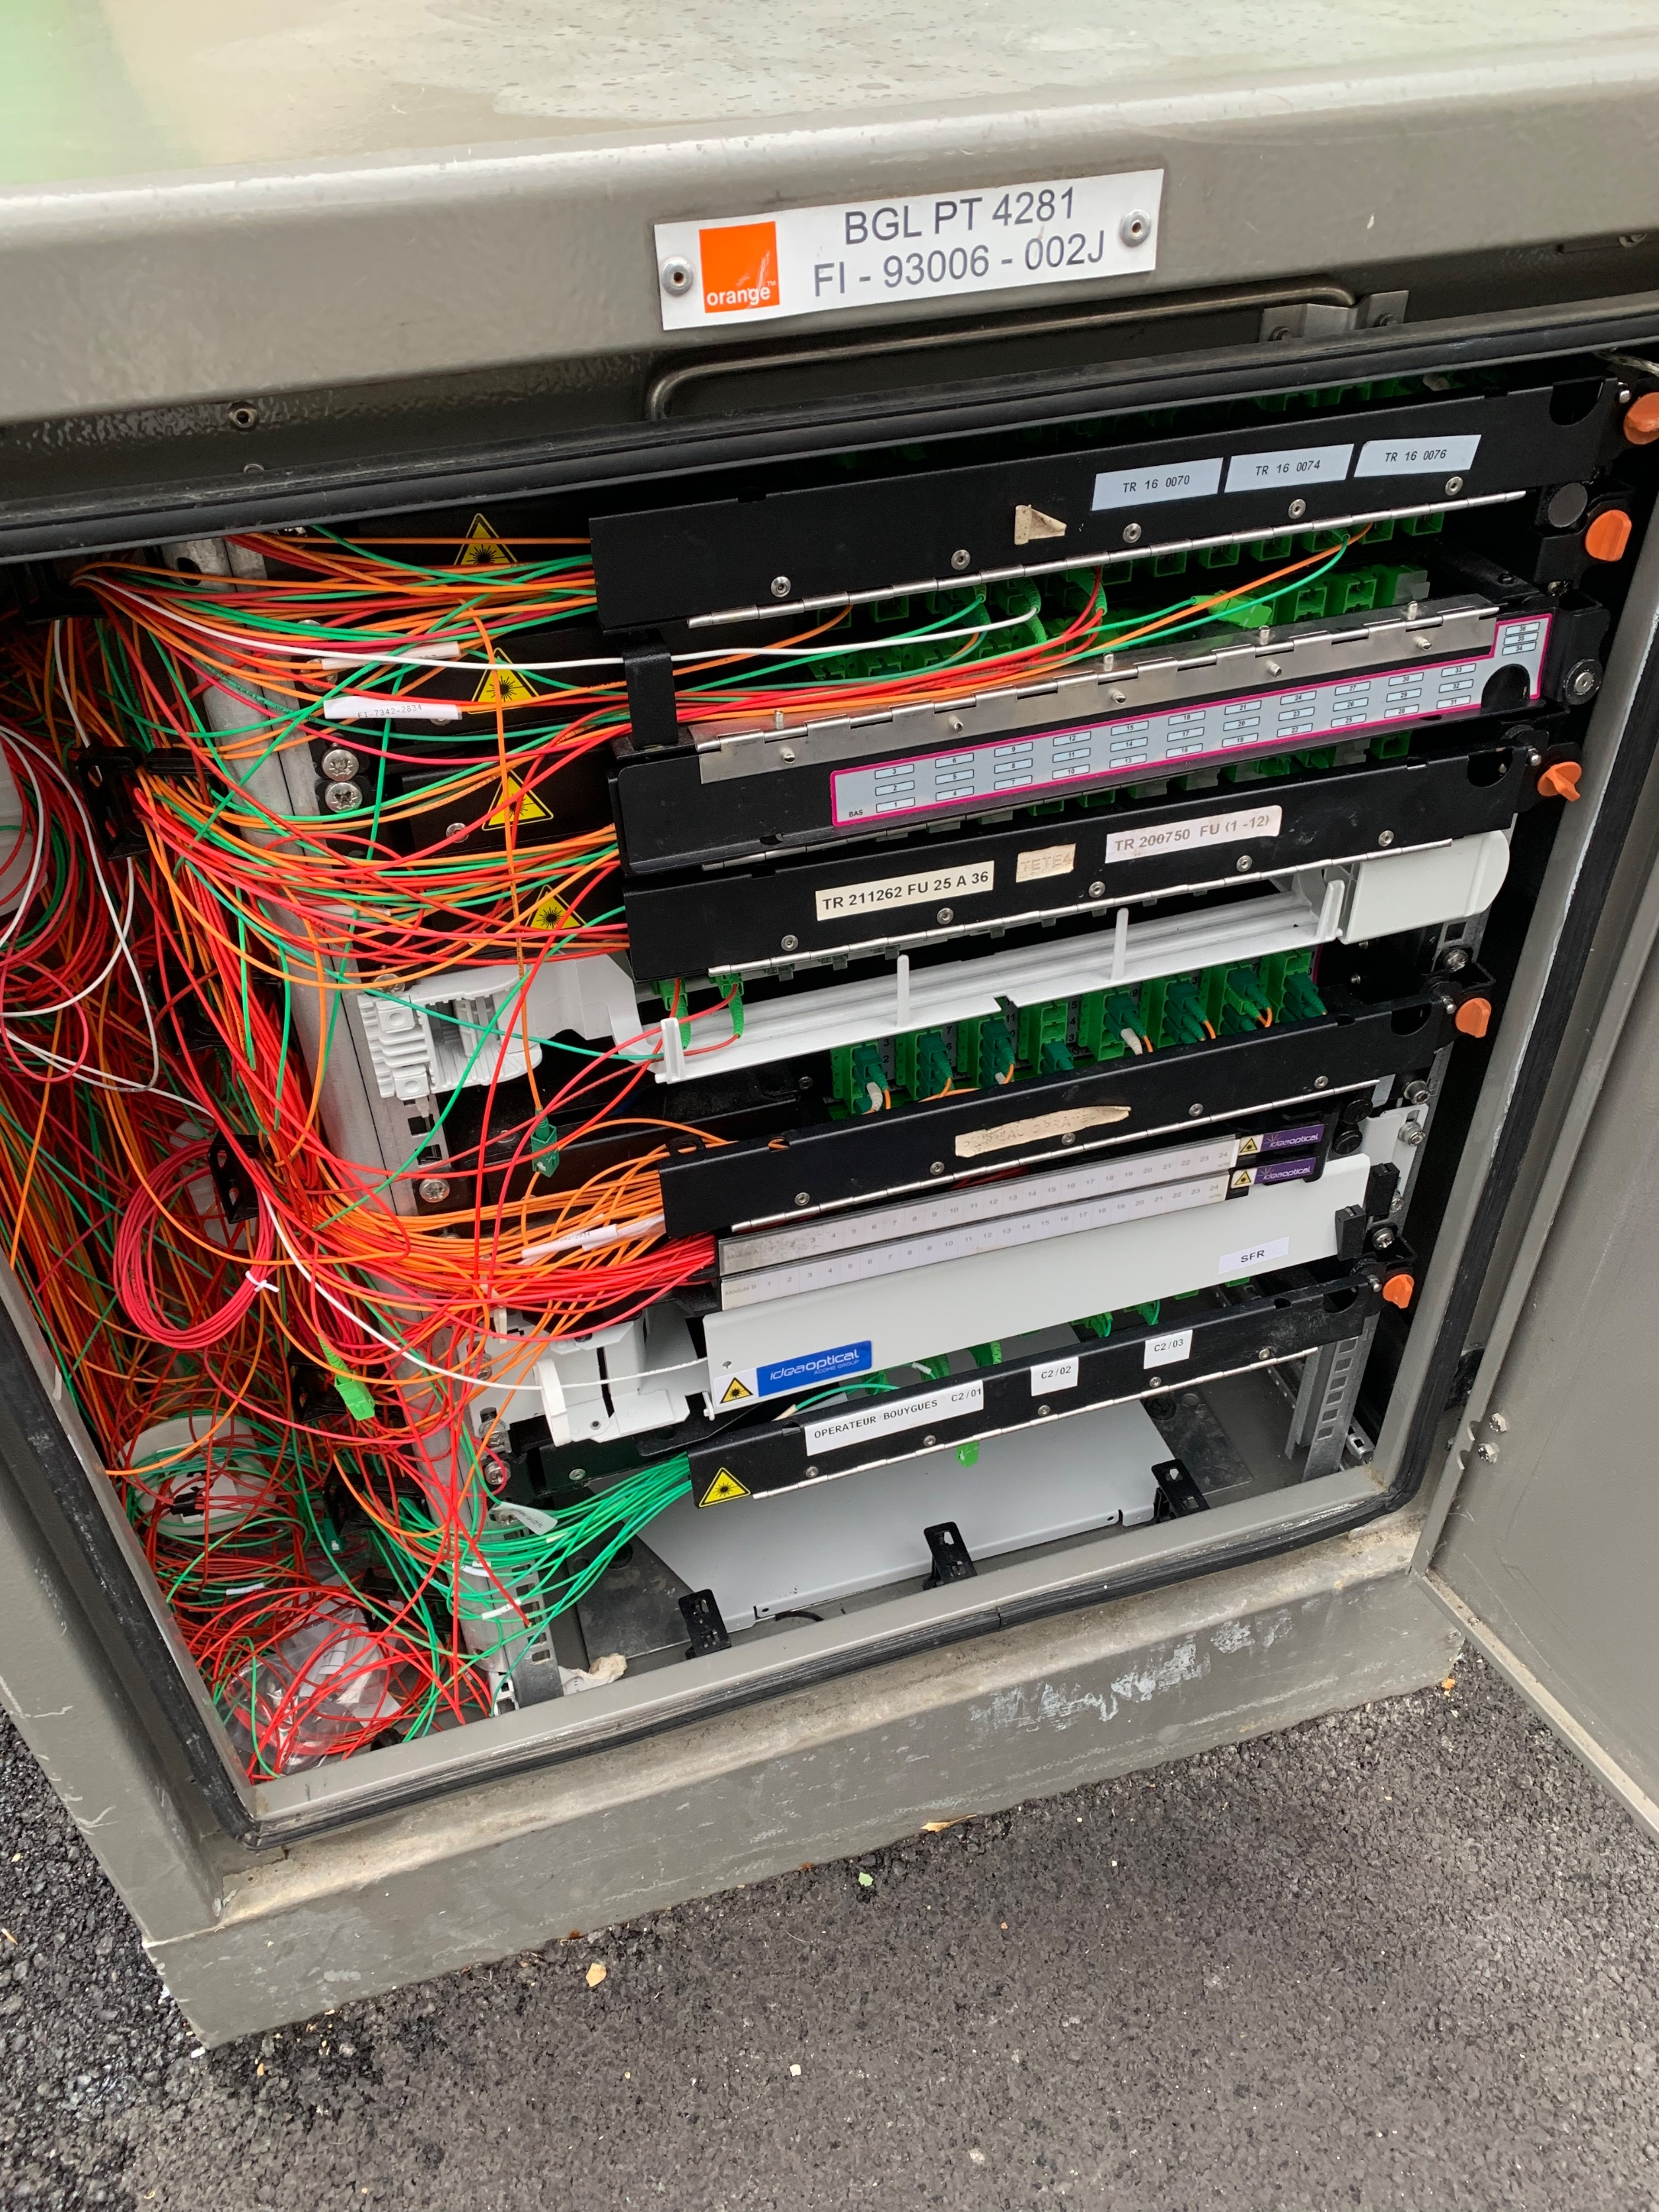
\includegraphics[width=\linewidth]{images/pm_example_3.jpg}
        \caption{PM no 3}
    \end{subfigure}
    \begin{subfigure}{0.5\textwidth}
        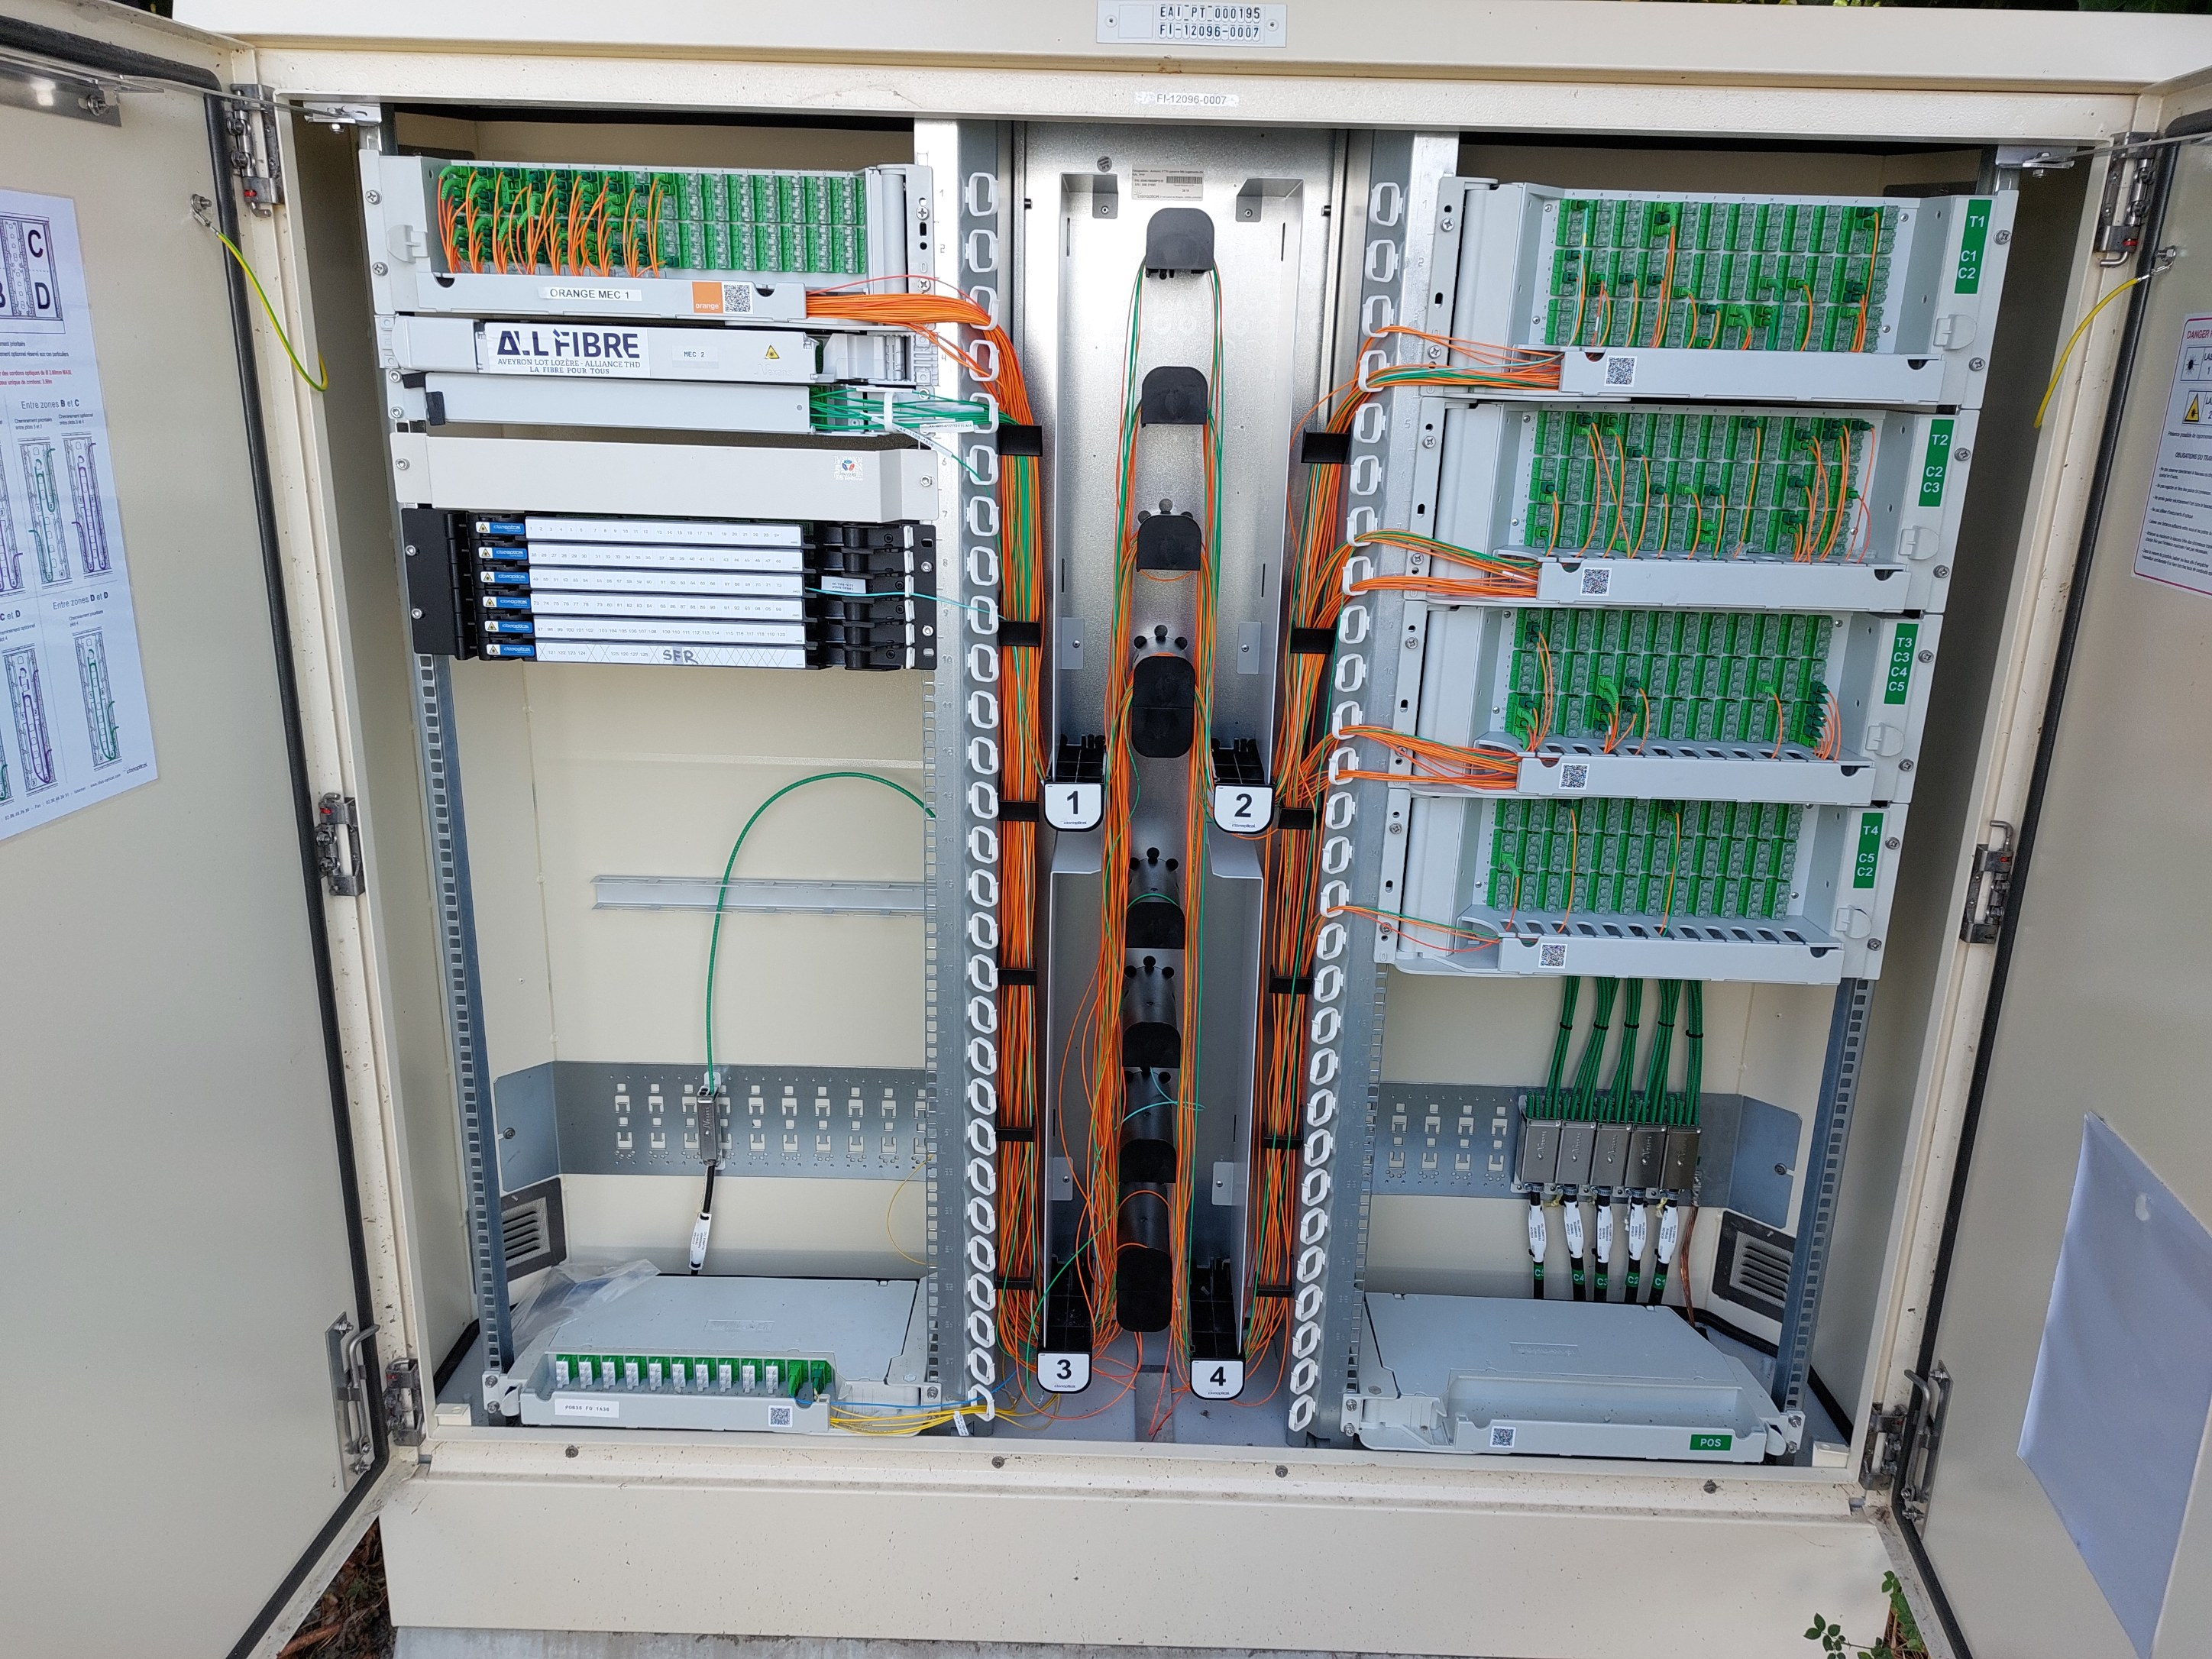
\includegraphics[width=\linewidth]{images/pm_example_4.jpg}
        \caption{PM no 4}
    \end{subfigure}
    \caption{Example of fiber distribution points}
    \label{fig:pm}
\end{figure}

Each point of the network is critical for the region in which it is located. With hundreds of thousands of points, it is difficult to do the maintenance and modernization of the network without collaborating with other companies or outsourcing it to third parties. The work on the fiber distribution point is processed by technicians who are not necessarily staff of SFR, but they could be also staff of such outsourcing companies and the operators will pay the fee for these companies or these independent technicians according to the workload.

To validate their work, an internal application has been used by the technicians to take a picture of their work and according to the image before and after of the fiber distribution point. However, although most of the technicians are honest, some of them do not. They could take a picture once and reupload their previous work several times in order to have validated several times.

It is necessary to build a system that can detect fake and near-duplicate images to prevent technicians from abusing the system. In 80\% of the reupload cases, technicians upload the same image that they have uploaded before. In this case, we could quickly resolve the problem by building a database of image fingerprints and comparing the fingerprints of the new images with it.

In the other 20\%, The images could be changed slightly by the technicians before re-uploading. It includes techniques following:

\begin{itemize}
    \item Slightly rotate the image
    \item Flip the image
    \item Put the image in slide a color box
\end{itemize}

It could be difficult for the system to use the exact image fingerprint because the images have been retouched. If we put the threshold too high, some of the forgery images will pass the system, and if the threshold is set too low, it will trigger false alarms.

The output of this project is to resolve this problem by using computer vision and deep learning techniques.

\subsection{Research the feasibility of moving the team's infrastructure to the Google Cloud}

In response to the evolving demands of a dynamic technological landscape, SFR Analytics is considering a shift from its existing local server infrastructure to a cloud-based model. This move aims to address current challenges and leverage the benefits offered by cloud computing.

The existing local server setup at SFR presents several challenges that impact efficiency, scalability, and operational agility. Moving infrastructure to Google Cloud offers a multitude of benefits that can significantly impact an organization's operations, scalability, and overall efficiency. Here are some key advantages of making this transition:


\begin{itemize}
    \item Scalability and Flexibility: Local servers are limited in their ability to scale on-demand, hindering the organization's ability to handle varying workloads effectively. Cloud services enable seamless scaling of resources, allowing SFR to adapt to changing workloads efficiently.
    
    \item High Costs: The capital expenditure associated with maintaining and upgrading local servers contributes to a significant financial burden. Cloud computing operates on a pay-as-you-go model, reducing upfront costs and minimizing ongoing maintenance expenses.

    \item Maintenance Complexity: Ongoing maintenance, updates, and troubleshooting of local servers require dedicated IT resources and time. Cloud providers handle infrastructure maintenance, updates, and security, freeing up internal IT resources.

    \item Limited Geographic Reach: Local servers may result in latency issues and slower performance for users across different regions. Cloud data centers strategically located worldwide ensure improved latency and enhanced user experiences. Cloud platforms offer built-in redundancy and disaster recovery capabilities, ensuring minimal downtime and data loss.
\end{itemize}

\textbf{Role in Cloud Migration:} Deploying ML and AI Models on Google Cloud Vertex AI

As a contributor to the migration of SFR's infrastructure to Google Cloud, my role revolves around the research of deployment of Machine Learning (ML) and Artificial Intelligence (AI) models on Google Cloud's Vertex AI platform. This initiative aligns with SFR's commitment to leveraging cutting-edge technologies to optimize operations and enhance customer experiences.

\begin{figure}[H]
    \centering
    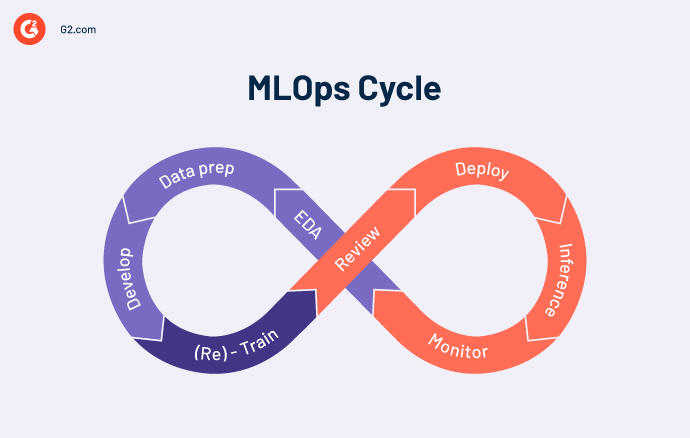
\includegraphics[width=0.7\textwidth]{images/G2CM_FI427_Learn_Article_[Machine_learning_operationalization]_Infographic_image1b_V1.png}
    \caption{MLOps cycle. source: G2.com}
    \label{fig:altice_campus}
\end{figure}

The current workflow of our team is surrounded by the usage of Airflow. The models right now run principally in R script, and we use Airflow to calculate the inferences of the model every day with the supervision of team members. However, some of the work is still manual, and the system stability has been show to be a question. Updating the models also faces differences with a lot of testing before pushing the new models to the production environment

With MLOps, we can solve multiple problems and have various advantages. The most important thing in the deployment of models is the model cycle. Once deployed, it could automatically fetch data needed for training or inference from the database, automatically clean the data and do the preprocessing procedure, automatically evaluate the performance of the new model, and finally automatically deploy the new model to the production environment if critical conditions surpass the set threshold.



\subsection{Apply machine learning techniques on call log from SFR's call center}

As an operator, SFR needs to listen to its customers to find the best and fastest way to improve its services in order to make it more competitive with its competitors. The mission of the customer care center is to listen to the needs of the customer and resolve customer problems that they cannot solve using the dashboard or our chatbot.

It is also essential for the company to understand the problems systematically. One of the ways to do that is to find the topic that is contained in each call from the customer to the call center. Currently, the agents who have the conversation with the customer or the agents who listen to these conversations do the labeling. The data analyst team finds patterns in such conversations and finds insight from such data. 

However, with the current technique of labeling, The conversations could be mislabeled because of the mistake of labelers, or simply because he or she doesn't understand fully the conversation and mislabels it. Therefore, it is necessary to build a system that could automatically detect the common theme of the corpus or suggest the main idea with a list of significant words of conversations.

The objective of the third mission is to use NLP techniques to find the common theme of given transcribed conversations, therefore facilitating the action of labelers with conversations. I will describe this mission in further detail since it is also the topic of the master thesis in the second part of this document.